\documentclass{rapportESPRIM}
\usepackage{setspace}
\setcounter{secnumdepth}{3}
\setcounter{tocdepth}{3}

\begin{document}
\renewcommand{\contentsname}{Table des Matières}
\pagenumbering{arabic}

\fairepagedegarde

% === Force a blank page after cover ===
\clearpage
\thispagestyle{empty}
\null
\clearpage

%-------------- Pages préliminaires --------------

\chapter*{Remerciements}
\addcontentsline{toc}{chapter}{Remerciements}
\setstretch{1.5}
Avant tout, je tiens à exprimer ma plus profonde gratitude à toutes celles et ceux qui m'ont soutenu tout au long de ce parcours vers l'obtention de mon diplôme d'ingénieur.

\textbf{À} ma famille bien-aimée, votre amour inébranlable, votre patience et vos encouragements ont été mon fondement. Cette réussite vous revient autant qu'à moi.

\textbf{Je} tiens à adresser mes sincères remerciements à mes encadrants et professeurs pour leurs conseils précieux, leur expertise et leur accompagnement tout au long de mon parcours académique. Leur dévouement a contribué à façonner l'ingénieur que je deviens.

\textbf{Un} remerciement particulier à l’ensemble du personnel administratif et technique qui a permis la concrétisation de ce programme. Votre soutien en coulisses a été crucial pour ma réussite.

\textbf{À} mes collègues et amis, merci pour les épreuves partagées et les moments de joie au cours de ce parcours exigeant mais enrichissant.

Ce diplôme d’ingénieur représente l’aboutissement d’un rêve de longue date, rendu possible grâce au soutien collectif de toutes les personnes mentionnées. Du fond du cœur, merci à vous tous.

\chapter*{Résumé}
\addcontentsline{toc}{chapter}{Résumé}
\setstretch{1.5}
Ce rapport présente le développement de \textbf{JourneyBuddy}, une application mobile innovante d’assistance au voyage basée sur l’IA, conçue pour aider les voyageurs à planifier efficacement leurs séjours. L’application exploite l’intelligence artificielle pour fournir des recommandations personnalisées, optimiser les itinéraires et offrir des informations de voyage en temps réel.

L'application Trip Assistant simplifie la planification grâce à l’automatisation de tâches complexes comme l’optimisation des parcours, les suggestions d’hébergement et la planification des activités. Grâce à l’intégration d’algorithmes d’apprentissage automatique, elle s’adapte aux préférences des utilisateurs et améliore progressivement ses suggestions.

Les fonctionnalités clés incluent la génération intelligente d’itinéraires, la planification en fonction du budget, les recommandations d’expériences locales et les mises à jour en temps réel des conditions de voyage. Cette application représente une avancée majeure dans la technologie du voyage, combinant utilité pratique et IA de pointe pour offrir une expérience de planification fluide.

Conçue avec une approche centrée sur l’utilisateur, Trip Assistant vise à réduire le stress lié à l’organisation des voyages tout en maximisant la satisfaction et l’efficacité du séjour. Ce projet démontre le potentiel des solutions basées sur l’intelligence artificielle pour transformer les secteurs traditionnels et améliorer concrètement l’expérience utilisateur.

%-------------- Table des matières --------------

\clearpage
\tableofcontents
\clearpage

\addcontentsline{toc}{chapter}{Liste des Figures}
\listoffigures
\clearpage

\addcontentsline{toc}{chapter}{Liste des Tableaux}
\listoftables
\clearpage

%------------ Corps du rapport ----------------

% CHAPTER 1: Étude Générale du Projet
\chapter{Étude Générale du Projet}
\section{Introduction}
Le premier chapitre met l'accent sur le contexte générale en commençant par la présentation de la société MOBELITE. Il s'ensuit la description du sujet à traiter, l'explication de la problématique de notre sujet. Par la suite nous allons étudier et critiquer des solutions existantes dans le marché international en proposant la solution envisagée et nous allons mentionner la méthodologie employée pour satisfaire les besoins des clients. 

\section{Présentation de l’Entreprise d’Accueil}

\subsection{Présentation Générale}

Mobelite est une digital factory créative spécialisée dans le développement de sites web et d’applications mobiles. Elle accompagne ses clients à chaque étape du projet, depuis la phase d’analyse des besoins jusqu’au déploiement final.

Les domaines d’expertise couvrent :
\begin{itemize}
    \item \textbf{Analyse des besoins :}Identification des fonctionnalités et contraintes nécessaires pour répondre aux attentes des utilisateurs.
    \item \textbf{Expérience utilisateur (UX) :}Conception d’interfaces ergonomiques, simples et engageantes.
    \item Conception et design : Création des maquettes et visuels pour structurer l’application de manière cohérente.
    \item \textbf{Développement web :} Réalisation de sites et applications accessibles via un navigateur.
    \item \textbf{Développement mobile multiplateforme (iOS/Android) :} Conception d’applications fonctionnant de manière fluide sur tous les types d’appareils.
    \item Architecture de services cloud : Mise en place d’infrastructures backend robustes et évolutives.
    \item \textbf{Intégration IA/ML dans les applications grand public :} Utilisation de l’intelligence artificielle pour proposer des expériences personnalisées.
    \item \textbf{Référencement naturel (SEO) :} Optimisation des contenus pour améliorer la visibilité sur les moteurs de recherche.
    \item \textbf{Déploiement (DevOps) :} Automatisation des processus de mise en production et gestion des versions.
    \item \textbf{Hébergement :} Mise en ligne et maintenance des services sur des serveurs fiables.
\end{itemize}

\subsection{Factory Web}

Mobelite conçoit des sites web modernes, intuitifs et responsives, compatibles avec tous les supports : ordinateurs, tablettes et mobiles.

\textbf{Expertises techniques :}
\begin{itemize}
    \item Développement de sites vitrines, applications web et plateformes interactives
    \item Maîtrise des technologies récentes : React JS, Node JS, Angular
    \item Approche centrée sur l’ergonomie et l’accessibilité
\end{itemize}

\subsection{Factory Mobile}

Mobelite développe des applications mobiles natives performantes, compatibles avec différents appareils et systèmes.

\textbf{Supports couverts :}
\begin{itemize}
    \item Smartphones et tablettes
    \item Montres connectées (Watch)
    \item Téléviseurs (TV connectées)
\end{itemize}

\textbf{Technologies maîtrisées :}
\begin{itemize}
    \item Développement natif sur iOS et Android
    \item Performance et adaptabilité multisupport
\end{itemize}

\subsection{Méthodologie Agile}

Mobelite adopte une approche Agile pour tous ses projets, permettant une plus grande flexibilité et une meilleure intégration du client dans le processus.

\textbf{Avantages de l’approche Agile :}
\begin{itemize}
    \item Itérations rapides avec livraisons fréquentes
    \item Tests réguliers pour valider les fonctionnalités
    \item Intégration continue des retours utilisateurs
    \item Collaboration étroite grâce à des outils partagés
\end{itemize}

Chaque projet est encadré par des \textbf{Product Owners} et \textbf{Scrum Masters certifiés}, assurant un suivi rigoureux.

\subsection{Points Forts de l’Approche Agile}

\begin{itemize}
    \item \textbf{1. Flexibilité :} Capacité d’adaptation des équipes aux évolutions du projet
    \item \textbf{2. Échanges :} Communication continue entre les intervenants
    \item \textbf{3. Livrables :} Versions exploitables dès les premières itérations
    \item \textbf{4. Tests :} Réalisation régulière de tests pour garantir la qualité
    \item \textbf{5. Services :} Mise à disposition d’un centre de services dédié
    \item \textbf{6. Maintenance :} Tierce maintenance applicative assurée après le déploiement
\end{itemize}

Forte de projets réussis, Mobelite est particulièrement bien positionnée pour concrétiser JourneyBuddy, alliant maîtrise technique et compréhension approfondie des attentes des voyageurs modernes.

\begin{figure}[h]
\centering

\includegraphics[width=0.6\textwidth]{logos/mobelite.png}
\caption{Logo de Mobelite}
\label{fig:mobelite}
\end{figure}

\newpage

\section{Contexte de l'étude}

\subsection{Objectifs de l'étude}

Cette étude vise à analyser l’écosystème actuel des applications de planification de voyages, en identifiant les limitations technologiques et fonctionnelles rencontrées par les solutions existantes. L’objectif global est de détecter les opportunités d’innovation pour créer une application plus performante et adaptée aux attentes des voyageurs modernes.

Les objectifs spécifiques de l’analyse sont les suivants :

\begin{itemize}
    \item \textbf{Identifier les acteurs clés} du marché de la planification de voyage assistée par l’intelligence artificielle.
    \item \textbf{Évaluer les approches technologiques} actuelles, en mettant en lumière leurs points forts et faiblesses.
    \item \textbf{Analyser l’expérience utilisateur}, notamment en termes de personnalisation, de convivialité et d’adaptabilité.
    \item \textbf{Déceler les lacunes du marché} pour proposer une solution innovante répondant aux besoins non satisfaits.
\end{itemize}

\subsection{Panorama des solutions existantes}

Le marché des planificateurs de voyage mobiles est actuellement dominé par plusieurs applications populaires qui offrent des services pratiques, mais dont les capacités restent limitées en matière d’intelligence contextuelle et de personnalisation parmi les applications les plus utilisées, nous pouvons citer: 

\paragraph{TripIt} est une application qui centralise automatiquement les réservations de voyage à partir des emails pour générer un itinéraire principal clair et consultable.

\begin{figure}[H]
\centering
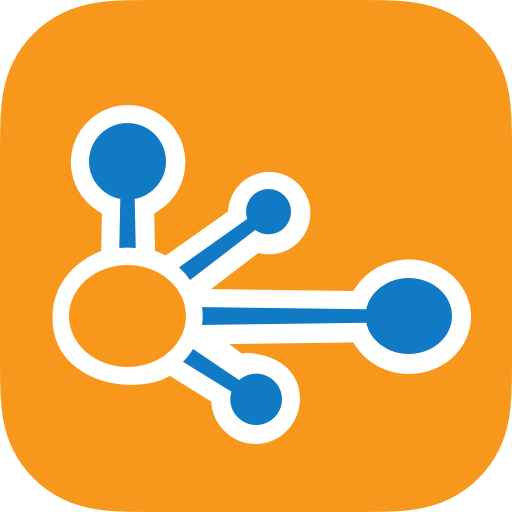
\includegraphics[width=0.3\textwidth]{logos/TripIT.png}
\caption{Logo de TripIt}
\end{figure}

\paragraph{TripAdvisor} est une plateforme riche en avis, notes et recommandations sur des destinations, hôtels, restaurants et attractions touristiques.

\begin{figure}[H]
\centering
\includegraphics[width=0.3\textwidth]{logos/tripadvisor.png}
\caption{Logo de TripAdvisor}
\end{figure}

\paragraph{Airbnb} met en relation les voyageurs avec des hôtes locaux, proposant à la fois hébergement et expériences personnalisées comme des activités ou des visites guidées.

\begin{figure}[H]
\centering

\includegraphics[width=0.3\textwidth]{logos/airbnb.png}
\caption{Logo d'Airbnb}
\end{figure}

Bien que ces plateformes soient fonctionnelles et reconnues, elles montrent des limites importantes concernant la personnalisation poussée, l'adaptabilité en temps réel et l’intégration de recommandations intelligentes basées sur l’IA.

\subsection{Analyse critique}

L’analyse approfondie des applications existantes met en lumière leurs forces, mais surtout les insuffisances que JourneyBuddy ambitionne de surmonter.

\paragraph{TripIt}
\begin{itemize}
    \item \textbf{Points forts :} Automatisation efficace de l’agrégation des réservations.
    \item \textbf{Limites :}
    \begin{itemize}
        \item Absence de personnalisation intelligente.
        \item Aucune gestion en temps réel des perturbations.
    \end{itemize}
\end{itemize}

\paragraph{TripAdvisor}
\begin{itemize}
    \item \textbf{Points forts :} Large base de recommandations communautaires.
    \item \textbf{Limites :}
    \begin{itemize}
        \item Forte dépendance aux avis parfois obsolètes.
        \item Manque de personnalisation dynamique.
    \end{itemize}
\end{itemize}

\paragraph{Airbnb}
\begin{itemize}
    \item \textbf{Points forts :} Offre immersive avec hébergement et expériences locales.
    \item \textbf{Limites :}
    \begin{itemize}
        \item Ne couvre pas la planification complète du voyage.
        \item Aucune gestion d’itinéraire ou de recommandations en fonction des imprévus.
    \end{itemize}
\end{itemize}

\section{Solution Proposée}

\subsection{Innovation de JourneyBuddy}

JourneyBuddy propose une nouvelle approche de la planification de voyage, fondée sur l’intelligence artificielle, l’apprentissage automatique et l’adaptabilité en temps réel. L’application vise à offrir une expérience fluide, intuitive et personnalisée.
\textbf{Fonctionnalités innovantes de JourneyBuddy :}
\begin{itemize}
    \item Recommandations contextuelles basées sur le machine learning.
    \item Moteur d’optimisation d’itinéraire dynamique et adaptatif.
    \item Interface conversationnelle intelligente via le traitement du langage naturel (NLP).
    \item Centralisation des réservations et synchronisation avec les plateformes partenaires.
    \item Détection des perturbations (ex. : météo, retards) et ajustement automatique.
\end{itemize}

Ces éléments placent JourneyBuddy à la croisée entre technologie, personnalisation et intelligence.

\subsection{Objectifs ciblés}

Pour mesurer l’impact et l’efficacité de JourneyBuddy, plusieurs indicateurs de performance ont été définis :

\begin{itemize}
    \item Réduire le temps moyen de planification de 70\% par l’automatisation intelligente.
    \item Atteindre un taux de satisfaction utilisateur de 90\% sur la qualité des recommandations.
    \item Couvrir plus de 50 destinations internationales dès la version initiale.
    \item Garantir un temps de réponse inférieur à une seconde pour chaque suggestion.
\end{itemize}

Ces objectifs soutiennent l’ambition de JourneyBuddy d’être un assistant de voyage intelligent de nouvelle génération.


\section{Processus de Développement}

\subsection{Méthodologie Agile}

La méthodologie Agile repose sur une approche itérative et incrémentale du développement logiciel. Elle favorise une adaptation rapide aux changements, une communication constante avec le client et une livraison continue de valeur.

\begin{figure}[H]
    \centering
    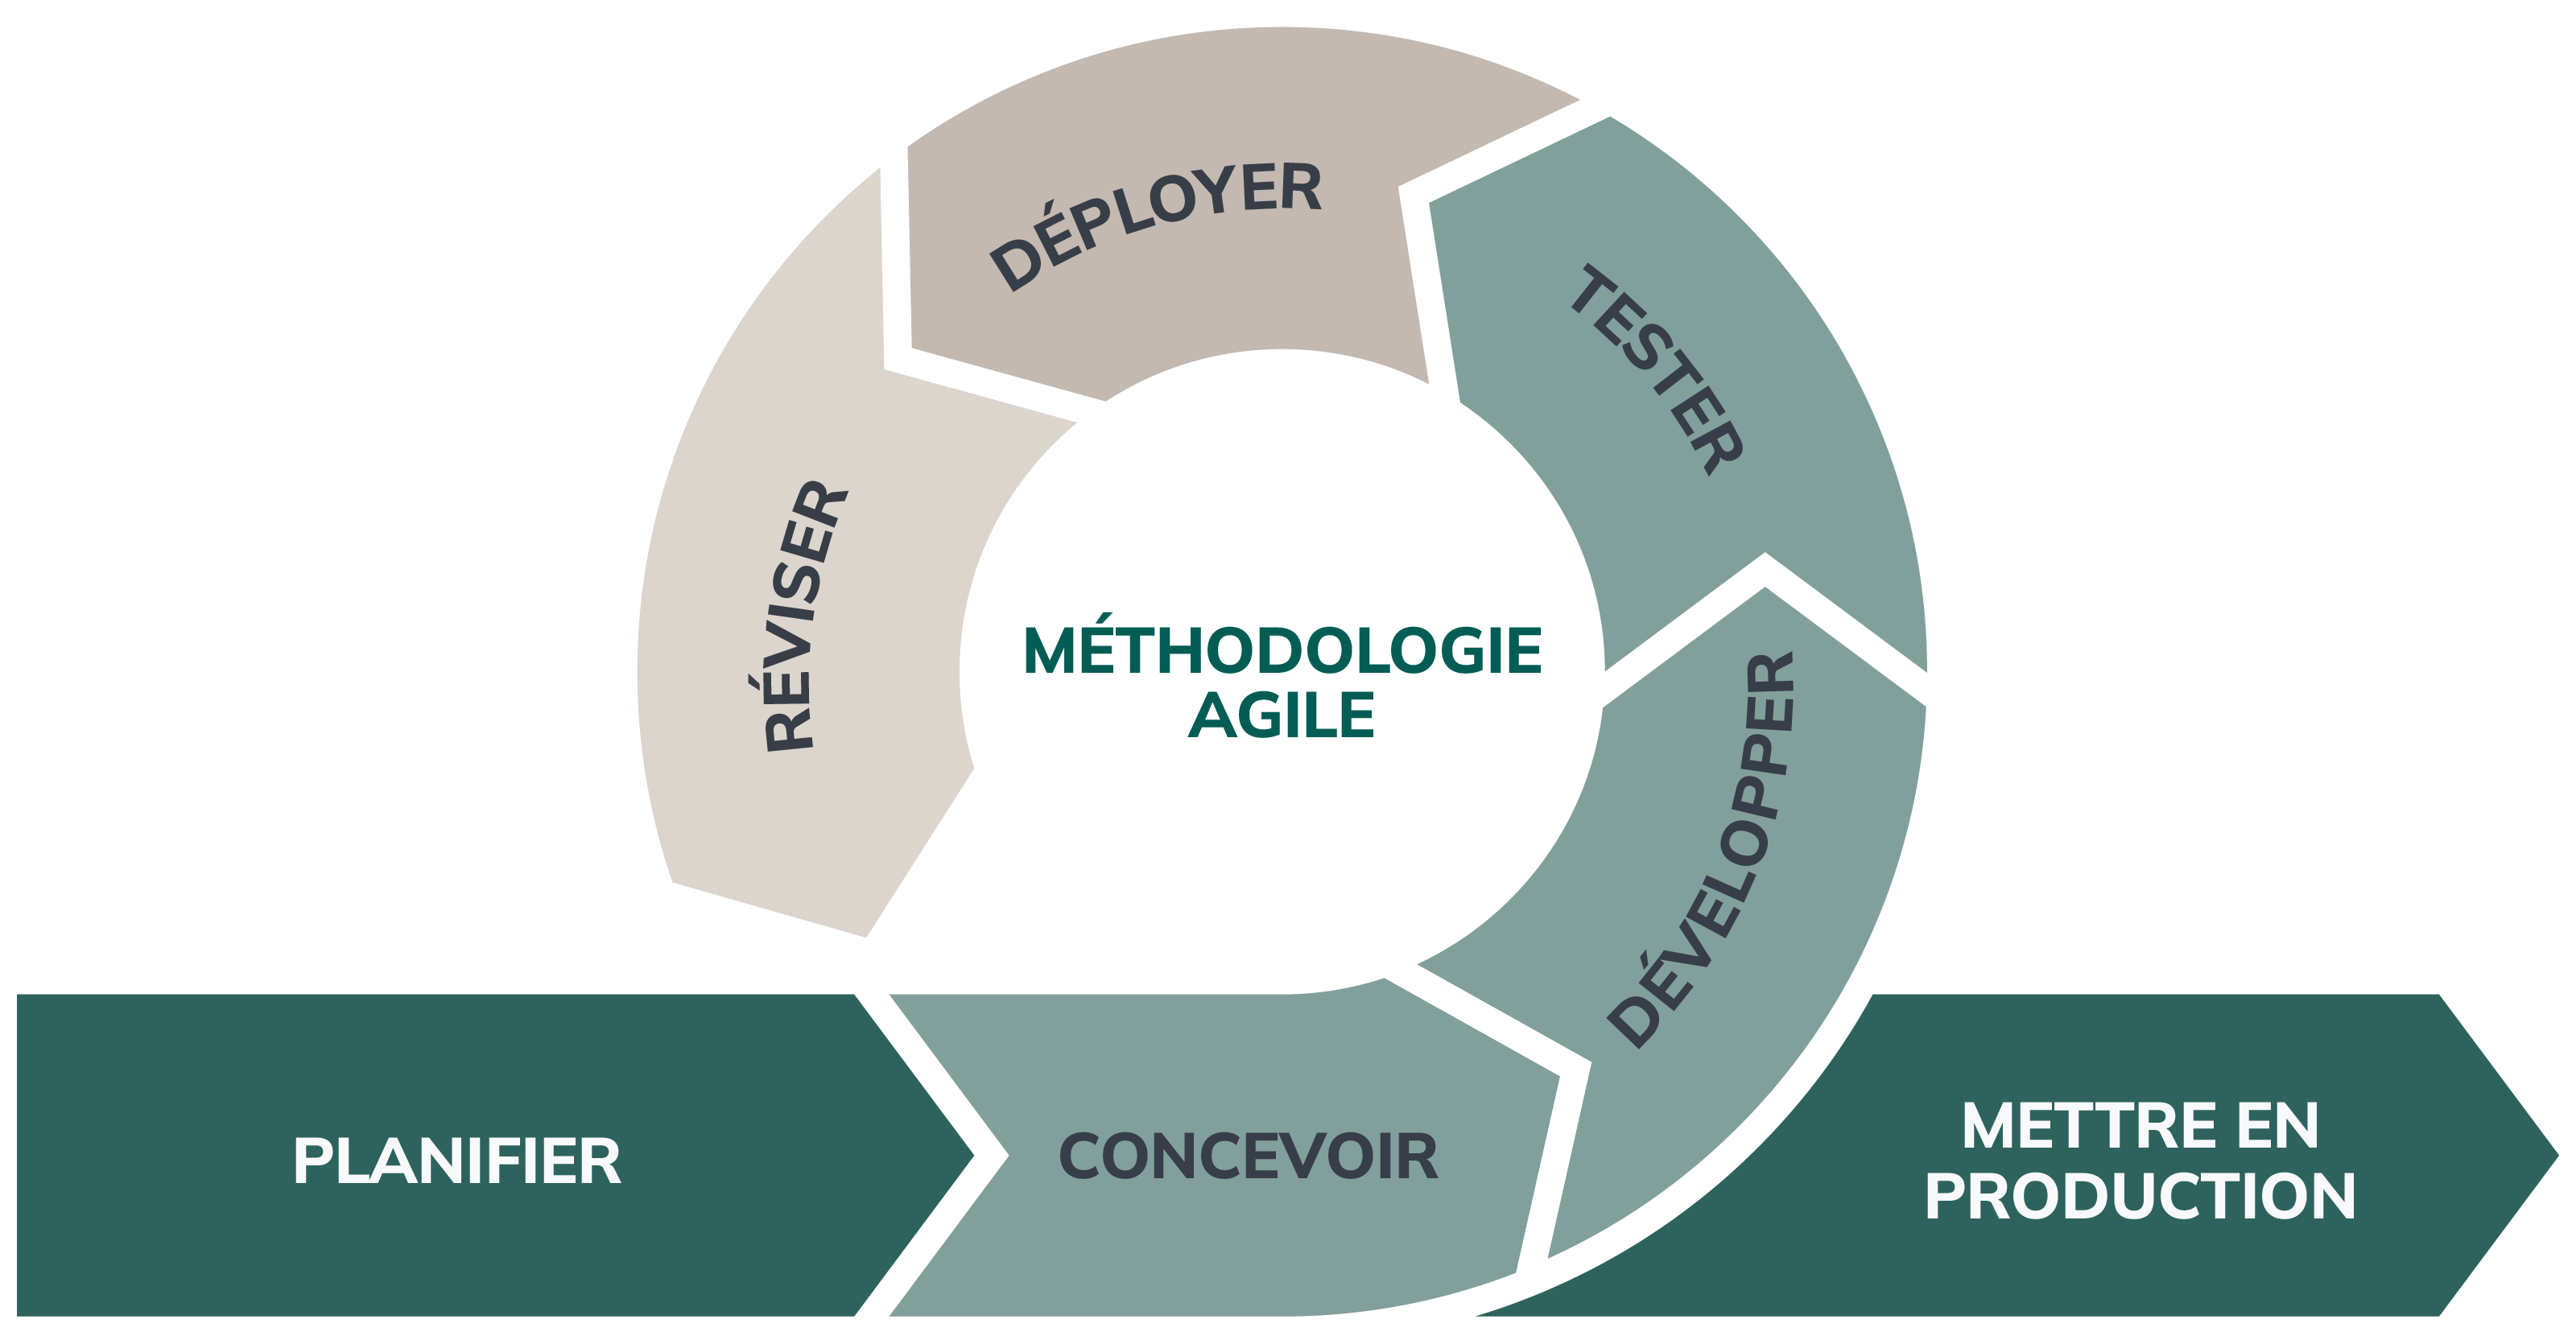
\includegraphics[width=0.8\textwidth]{figures/agile.png} % Remplace avec ton chemin d'image
    \caption{Cycle de développement Agile}
    \label{fig:agile-method}
\end{figure}

\subsection{Les principes de l’agilité}

Les principes de l’agilité mettent l’accent sur la satisfaction du client, l’adaptation au changement, la collaboration continue, et la livraison fréquente de produits fonctionnels. Ces principes sont fondamentaux dans le cadre du projet JourneyBuddy.

\subsection{Méthodologie Scrum}

La méthodologie Scrum est une mise en œuvre concrète de l’approche Agile. Elle se structure autour de rôles, d’événements, et d’artéfacts spécifiques qui organisent le travail de l’équipe de manière itérative.

\begin{figure}[H]
    \centering
    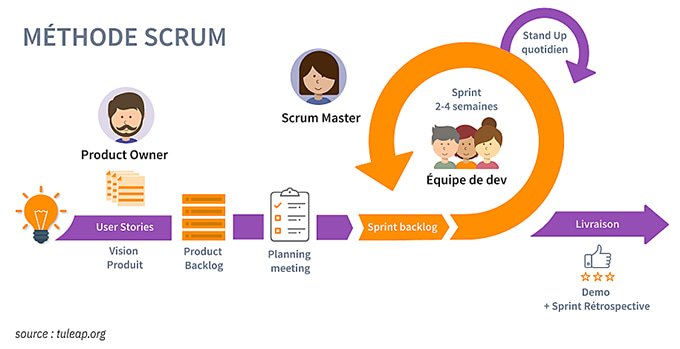
\includegraphics[width=0.8\textwidth]{figures/scrum.jpg} % Remplace avec ton chemin d'image
    \caption{Modélisation de la méthode SCRUM}
    \label{fig:scrum-method}
\end{figure}

\subsubsection{Pourquoi choisir la méthode Scrum ?}

Scrum offre une grande flexibilité, une communication continue, et une capacité à produire rapidement de la valeur tout en intégrant les retours des utilisateurs.

\textbf{Le backlog du produit}

Il s’agit d’une liste hiérarchisée de toutes les fonctionnalités souhaitées dans le produit. Elle est gérée par le Product Owner et régulièrement réévaluée.

\textbf{Les intervenants dans Scrum :}
\begin{itemize}
    \item \textbf{Product Owner} : Responsable de la définition des besoins et du backlog produit.
    \item \textbf{Scrum Master} : Garant du bon respect des règles Scrum, facilite les réunions et supprime les obstacles.
    \item \textbf{Développeurs} : Conçoivent, développent et testent les fonctionnalités au sein des sprints.
\end{itemize}

\textbf{Le Sprint}

Un sprint est une période fixe, généralement de deux semaines, durant laquelle une partie du produit est développée et rendue fonctionnelle. Chaque sprint se termine par une démonstration et une rétrospective.

\subsubsection{Adaptation de la méthodologie Scrum dans le projet}

\textbf{Nos intervenants :}
\begin{itemize}
    \item \textbf{Scrum Master} : Samia Ben Ismail
    \item \textbf{Product Owner} : Amina Dgham
    \item \textbf{Développeurs} : Amira Boubaker, Amer  Akrimi
\end{itemize}

\textbf{Product Backlog :}
\begin{table}[H]
    \centering
    \begin{tabularx}{\textwidth}{|c|X|c|}
        \hline
        \textbf{PBI} & \textbf{User Story} & \textbf{Priorité} \\
        \hline
        PB1 & En tant qu’utilisateur, je veux créer un compte pour personnaliser mon expérience. & Haute \\
        \hline
        PB2 & En tant qu’utilisateur, je veux m’authentifier afin d’accéder à mon espace personnel. & Haute \\
        \hline
        PB3 & En tant qu’utilisateur, je veux consulter les points d’intérêts disponibles. & Haute \\
        \hline
        PB4 & En tant qu’utilisateur, je veux filtrer les points d’intérêts selon des critères. & Moyenne \\
        \hline
        PB5 & En tant qu’utilisateur, je veux consulter les alertes d’événements culturels internationaux. & Moyenne \\
        \hline
        PB6 & En tant qu’utilisateur, je veux chercher un point d’intérêt par lettre alphabétique. & Basse \\
        \hline
        PB7 & En tant qu’utilisateur, je veux créer une carte de voyage soit sans, soit avec assistance AI. & Haute \\
        \hline
        PB8 & En tant qu’utilisateur, je veux chercher un vol correspondant à mon départ et arrivée avec les bonnes dates. & Haute \\
        \hline
        PB9 & En tant qu’utilisateur, je veux chercher un hôtel dans la même ville d’arrivée. & Haute \\
        \hline
        PB10 & En tant qu’utilisateur, je veux choisir le type d’accompagnant pour mon voyage. & Moyenne \\
        \hline
        PB11 & En tant qu’utilisateur, je veux saisir un budget et calculer automatiquement le montant restant. & Haute \\
        \hline
        PB12 & En tant qu’utilisateur, je veux choisir l’activité la plus proche ou la filtrer par catégorie (avec assistance AI). & Moyenne \\
        \hline
        PB13 & En tant qu’utilisateur, je veux consulter les détails du voyage avant de l’enregistrer. & Haute \\
        \hline
    \end{tabularx}
\end{table}

\begin{table}[H]
    \centering
    \begin{tabularx}{\textwidth}{|c|X|c|}
        \hline
        PB14 & En tant qu’utilisateur, je veux enregistrer ma carte de voyage. & Haute \\
        \hline
        PB15 & En tant qu’utilisateur, je veux gérer ma carte de voyage & Moyenne \\
        \hline
        PB16 & En tant qu’utilisateur, je veux consulter mon historique de cartes de voyages. & Basse \\
        \hline
        PB17 & En tant qu’utilisateur, je veux ajouter un nouveau voyage soit sans, soit avec assistance AI. & Haute \\
        \hline
        PB18 & En tant qu’utilisateur, je veux visualiser la ville d’arrivée sur une carte interactive avec Google Maps. & Haute \\
        \hline
        PB19 & En tant qu’utilisateur, je veux modifier mes informations de profil (photo, téléphone, ville/pays, bio, adresse, mot de passe). & Moyenne \\
        \hline
        PB20 & En tant qu’utilisateur, je veux gérer mes favoris pour les points d’intérêts. & Moyenne \\
        \hline
        PB21 & En tant qu’utilisateur, je veux activer ou désactiver mes préférences. & Basse \\
        \hline
        PB22 & En tant qu’utilisateur, je veux changer le thème de l’application (clair/sombre). & Basse \\
        \hline
        PB23 & En tant qu’utilisateur, je veux me déconnecter de l’application. & Haute \\
        \hline
    \end{tabularx}
    \caption{Product Backlog de JourneyBuddy}
\end{table}

\textbf{Les Sprints :}
Chaque sprint est planifié selon la priorité du backlog, et vise une livraison incrémentale d’un produit utilisable.

\begin{figure}[H]
    \centering
    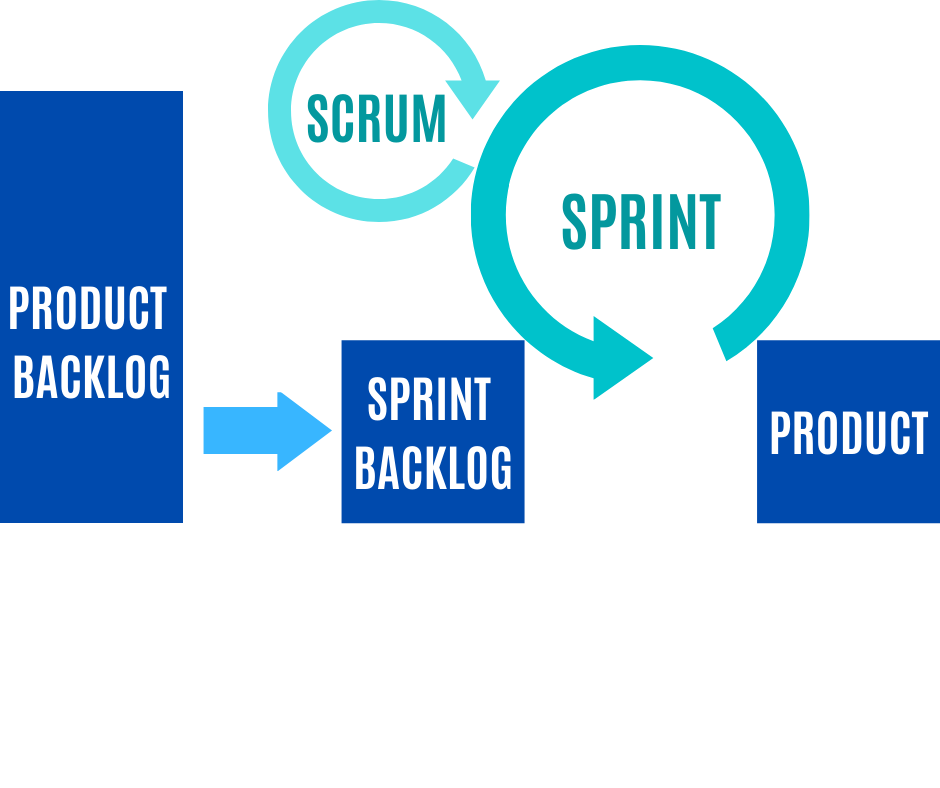
\includegraphics[width=0.7\textwidth]{figures/scrum-sprint.png} % Remplace avec ton image réelle
    \caption{Cycle de vie d’un Sprint Scrum}
    \label{fig:sprint-cycle}
\end{figure}

\begin{table}[H]
    \centering
    \begin{tabular}{|c|c|}
        \hline
        \textbf{Numéro de Sprint} & \textbf{Nom du Sprint} \\
        \hline
        Sprint 1 & Création du compte et Authentification \\
        \hline
        Sprint 2 & Planification de voyage et carte interactive \\
        \hline
        Sprint 3 & Suggestions IA et Chatbot intelligent \\
        \hline
        Sprint 4 & Finalisation UX/UI et Intégration Docker \\
        \hline
    \end{tabular}
    \caption{Découpage des Sprints pour JourneyBuddy}
    \label{tab:sprints}
\end{table}

\section{Conclusion}

Cette étude préliminaire met en lumière le potentiel de JourneyBuddy pour réinventer la planification de voyage. En se basant sur l’intelligence artificielle et une architecture agile, l’application promet une expérience personnalisée, fluide et réactive.

L’analyse du marché révèle des lacunes importantes que JourneyBuddy est capable de combler : personnalisation poussée, gestion intelligente des imprévus, et interface conversationnelle.

Grâce aux compétences techniques de l’équipe Mobelite, à son expertise en développement mobile et à l’application rigoureuse de la méthodologie SCRUM, le projet est bien positionné pour répondre aux attentes du marché.

\textbf{Prochaines étapes :}
\begin{itemize}
    \item Rédaction des spécifications techniques.
    \item Optimisation de l’expérience utilisateur.
    \item Lancement du prototype et itérations selon les retours utilisateurs.
\end{itemize}

JourneyBuddy ambitionne ainsi de devenir un compagnon de voyage incontournable dans l’ère numérique.


% CHAPTER 2: Analyse et Spécification des Besoins
\chapter{Analyse et Spécification des Besoins}
\section{Introduction}

Dans ce chapitre, nous détaillons l’analyse et la spécification des besoins fonctionnels et non fonctionnels de l’application \textit{JourneyBuddy}.  
Nous avons choisi la méthodologie agile SCRUM comme démarche de gestion de projet, favorisant un développement itératif et incrémental.  
Ce chapitre présente d'abord les exigences à satisfaire, puis l’environnement de travail retenu ainsi que les architectures générales adoptées (système et applicative).  
Enfin, nous clôturons par la planification générale de notre sprint, incluant les priorités, risques, et cas d’utilisation globaux.

\section{Analyse des besoins}

\subsection{Identification des besoins fonctionnels}

L’application est destinée à des voyageurs qui souhaitent planifier des itinéraires complets à l’aide d’une intelligence artificielle, incluant la réservation de vols, d’hôtels et d’activités touristiques.  
Les besoins fonctionnels définissent les fonctionnalités principales à implémenter telles que :

\begin{itemize}
    \item Création et gestion de compte utilisateur.
    \item Planification de voyage multi-étapes.
    \item Recherche intelligente de vols, hôtels et activités.
    \item Suggestions automatiques basées sur les préférences.
    \item Visualisation d’itinéraires.
\end{itemize}

\subsection{Identification des besoins non fonctionnels}

Les exigences non fonctionnelles portent sur :

\begin{itemize}
    \item \textbf{Performance} : temps de réponse acceptable même en cas de forte charge.
    \item \textbf{Sécurité} : protection des données utilisateurs (authentification, HTTPS...).
    \item \textbf{Accessibilité} : compatibilité multiplateforme via React Native.
    \item \textbf{Scalabilité} : architecture permettant l’extension future des services.
\end{itemize}

\section{Planification du traitement des cas d'utilisation}

Nous avons planifié les différentes fonctionnalités à travers un backlog produit en lien avec les cas d’utilisation, en tenant compte des priorités et des risques potentiels.

\subsection{Priorité}

\begin{itemize}
    \item \textbf{Haute} : fonctionnalités essentielles au fonctionnement de base.
    \item \textbf{Moyenne} : fonctionnalités utiles mais non critiques.
    \item \textbf{Basse} : compatibilité multiplateforme via React Native.
    \item \textbf{Scalabilité} : ajouts secondaires ou esthétiques.
\end{itemize}

\subsection{Risques}

Certains éléments du projet présentent des risques potentiels à anticiper :

\begin{itemize}
    \item Dépendance à des API externes (fluctuations, indisponibilité).
    \item Volume de données à gérer en base.
    \item Complexité de l’algorithme de recommandation.
\end{itemize}

\subsection{Diagramme de cas d'utilisation globale}

\begin{figure}[H]
    \centering
    \includegraphics[width=0.9\textwidth]{usecases/usecase}
    \caption{Diagramme de cas d'utilisation global de JourneyBuddy}
\end{figure}

\section{Description de l'application}

L’application \textbf{JourneyBuddy} est une application mobile construite avec la stack \textbf{MERN} :

\begin{itemize}
    \item \textbf{Frontend} en React Native, pour développer une interface utilisateur native sur iOS et Android.
    \item \textbf{Backend} en Node.js et Express.js, pour gérer la logique métier et les routes.
    \item \textbf{Base de données} MongoDB, orientée documents, idéale pour stocker des données flexibles et évolutives.
\end{itemize}

\subsection{Environnement de Travail}

Le projet adopte la stack MERN, qui combine MongoDB, Express, React Native et Node.js. Cette architecture permet un développement complet (frontend + backend) en JavaScript, favorisant la rapidité et la cohérence.

\begin{figure}[H]
    \centering
    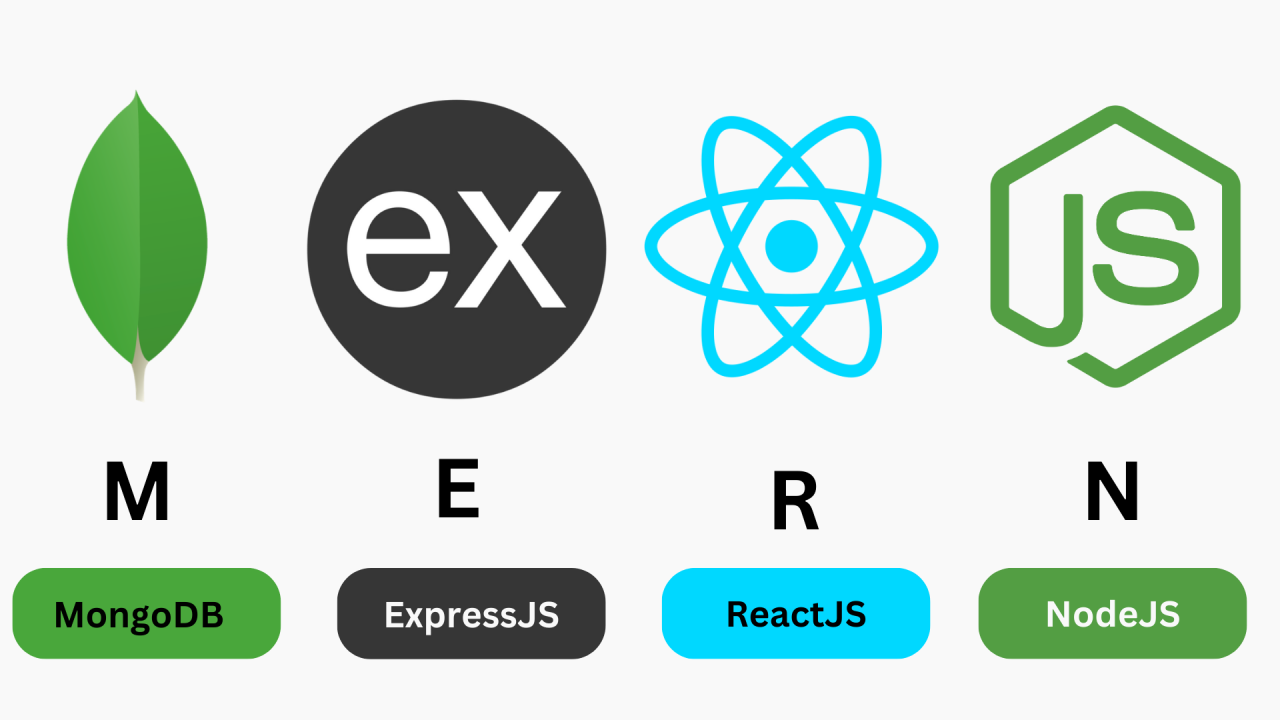
\includegraphics[width=0.7\textwidth]{logos/mern.png}
    \caption{Architecture MERN choisie}
\end{figure}

\renewcommand{\thesubsubsection}{\thesubsection.\arabic{subsubsection}} % Active la numérotation des subsubsection

\subsubsection{1. Outils de Développement et Modélisation}

\begin{itemize}
    \item \textbf{Visual Studio Code} : éditeur principal pour le développement de code.
    \begin{figure}[H]
        \centering
        
\includegraphics[width=0.5\textwidth]{logos/vscode.png}
        \caption{Environnement de développement : VS Code}
    \end{figure}

    \item \textbf{Visual Paradigm} : outil de modélisation UML et de conception visuelle utilisé pour l’analyse, la conception et la documentation des systèmes logiciels.
    \begin{figure}[H]
        \centering
        
\includegraphics[width=0.5\textwidth]{logos/visualparadigm.png}
        \caption{Outil de modélisation : Visual Paradigm}
    \end{figure}

    \item \textbf{Docker} : plateforme de conteneurisation permettant d’empaqueter des applications et leurs dépendances dans des conteneurs légers, portables et reproductibles.
    \begin{figure}[H]
        \centering
        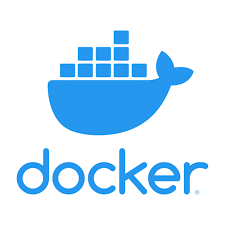
\includegraphics[width=0.3\textwidth]{logos/docker.png}
        \caption{Docker - Conteneurisation et virtualisation légère}
    \end{figure}

    \item \textbf{Docker Hub} : registre public officiel de Docker, permettant d’héberger, de partager et de télécharger des images de conteneurs.
    \begin{figure}[H]
        \centering
        
\includegraphics[width=0.3\textwidth]{logos/dockerhub.png}
        \caption{Docker Hub - Registre d’images de conteneurs}
    \end{figure}
\end{itemize}

\subsubsection{2. Plateforme de Développement}

\begin{itemize}
    \item \textbf{MongoDB Atlas} : base de données cloud sécurisée pour héberger les données.
    \begin{figure}[H]
        \centering
        
\includegraphics[width=0.5\textwidth]{logos/mongodb-atlas.png}
        \caption{MongoDB Atlas - Plateforme de base de données cloud}
    \end{figure}

    \item \textbf{MongoDB Compass} : interface graphique pour la visualisation et la manipulation des collections MongoDB.
    \begin{figure}[H]
        \centering
        
\includegraphics[width=0.7\textwidth]{logos/mongodb-compass.png}
        \caption{MongoDB Compass - Outil de gestion des collections}
    \end{figure}
\end{itemize}

\subsubsection{3. Frameworks Utilisés}

\paragraph{React Native} est un framework open-source développé par Meta permettant de créer des applications mobiles natives en JavaScript, facilitant ainsi le développement multiplateforme.

\begin{figure}[H]
    \centering
    
\includegraphics[width=0.3\textwidth]{logos/react-native.png}
    \caption{Framework React Native}
\end{figure}

\textbf{Avantages de React Native :}
\begin{itemize}
    \item Code partagé entre iOS et Android.
    \item Large communauté active et support continu.
    \item Performances proches du natif.
    \item Intégration aisée avec des API tierces.
\end{itemize}

\paragraph{Node.js et Express} forment un duo performant pour créer une API RESTful efficace. Node.js offre un environnement d'exécution côté serveur, tandis qu'Express fournit une structure légère pour la gestion des routes et des middlewares.

\begin{figure}[H]
    \centering
    
\includegraphics[width=0.25\textwidth]{logos/nodejs.png}
    \hspace{0.05\textwidth}
    
\includegraphics[width=0.25\textwidth]{logos/express.png}
    \caption{Node.js (à gauche) et Express (à droite)}
\end{figure}

\subsubsection{4. Langages Utilisés}

\begin{itemize}
    \item \textbf{TypeScript} : surensemble typé de JavaScript permettant de détecter les erreurs à la compilation.
    \begin{figure}[H]
        \centering
        \includegraphics[width=0.25\textwidth]{logos/typescript.png}
        \caption{Langage TypeScript}
    \end{figure}
\end{itemize}

\section{Architecture Adoptée}

L’architecture choisie définit la structure logicielle du système, garantissant modularité, maintenabilité et évolutivité.

\subsection{Architecture Système}
\setcounter{secnumdepth}{3}
% \hspace{0.2cm}
\subsubsection{Architecture 2-Tiers}
\setcounter{secnumdepth}{3}

L'architecture 2-Tiers repose sur une structure client-serveur classique, dans laquelle l'interface utilisateur (client) communique directement avec le serveur de base de données. Ce modèle est simple à implémenter et adapté aux applications légères, mais il présente des limitations en termes de scalabilité et de séparation des responsabilités.

\begin{figure}[H]
    \centering
    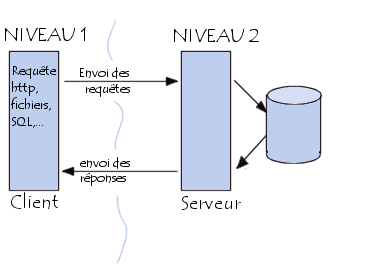
\includegraphics[height=0.4\textheight, width=0.7\textwidth]{figures/2-tier.png}
    \caption{Architecture 2-Tiers : client-serveur}
\end{figure}

\subsubsection{Architecture N-Tiers}

L'architecture N-Tiers introduit plusieurs couches logiques (présentation, logique métier, accès aux données, etc.), chacune jouant un rôle distinct. Cette séparation améliore la modularité, la sécurité et la maintenabilité, en facilitant les tests et l’évolution du système. Elle est particulièrement adaptée aux applications complexes à fort volume de données.

\begin{figure}[H]
    \centering
    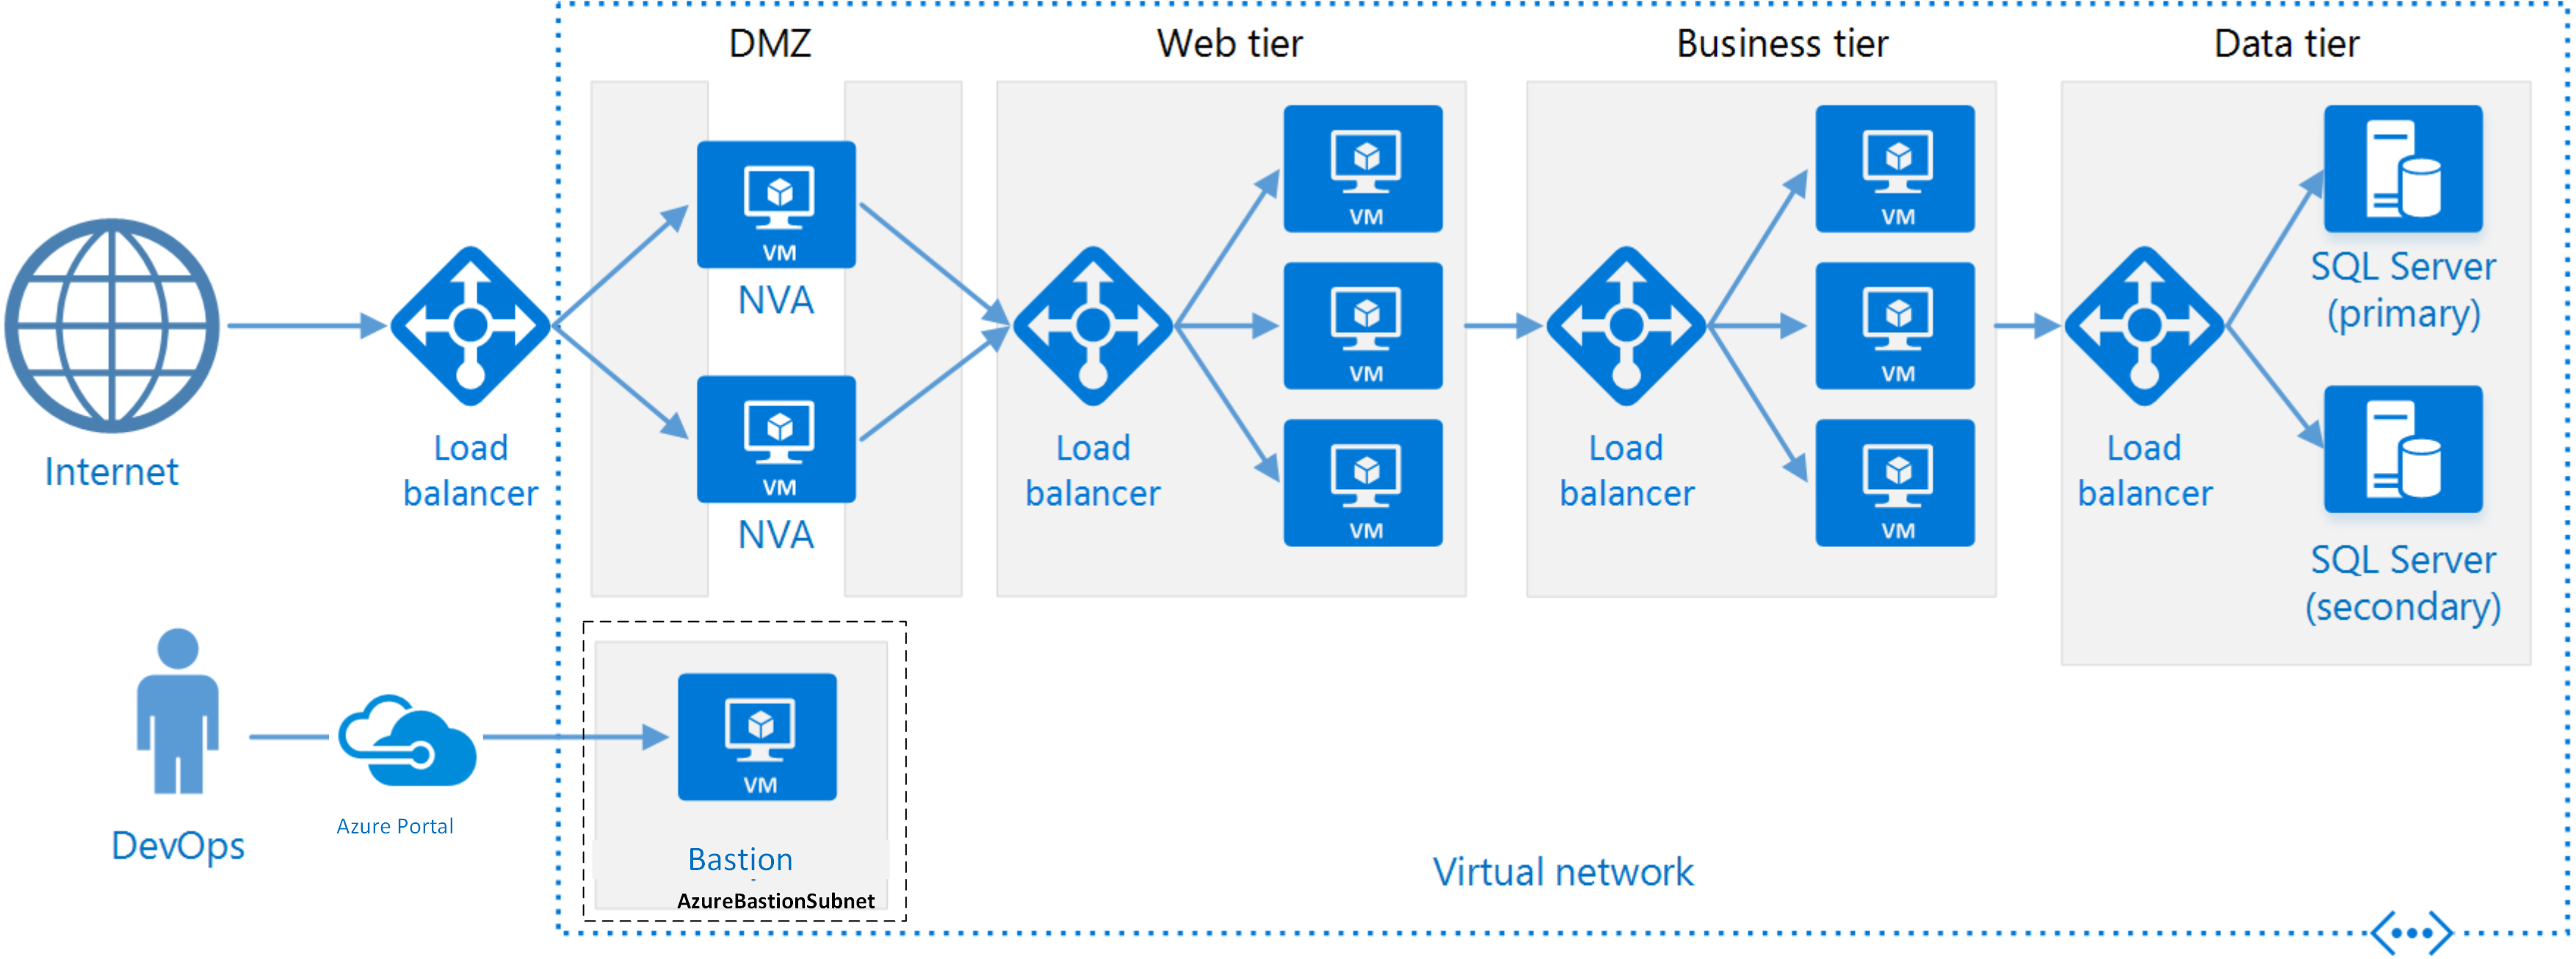
\includegraphics[height=0.4\textheight, width=0.9\textwidth]{figures/n-tier-arch.png}
    \caption{Architecture N-Tiers avec séparation logique en couches}
\end{figure}

\subsubsection{Architecture Adoptée : 3-Tiers}

JourneyBuddy adopte une architecture 3-Tiers, qui constitue une forme spécialisée de l’architecture N-Tiers. Elle se compose de trois couches principales :
\begin{itemize}
    \item \textbf{La couche présentation (frontend)} : gérée via React Native, elle gère les interfaces utilisateurs.
    \item \textbf{La couche logique métier (backend)} : assurée par Node.js et Express, elle traite les règles métiers et les requêtes.
    \item \textbf{La couche données} : gérée par MongoDB, elle stocke et fournit les informations.
\end{itemize}
Cette approche offre un excellent équilibre entre complexité, performance et évolutivité.

\newpage
\begin{figure}[H]
    \centering
    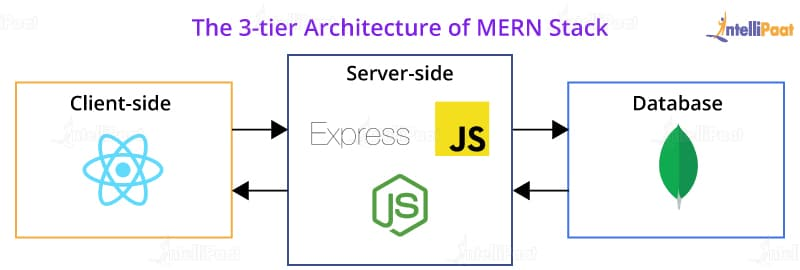
\includegraphics[width=0.8\textwidth]{figures/The-3-tier-Architecture-of-MERN-Stack.png}
    \caption{Architecture 3-Tiers retenue pour JourneyBuddy}
\end{figure}

\subsection{Architecture de l’application}

L'application suit le modèle MVC (Modèle – Vue – Contrôleur), une architecture classique permettant de séparer la gestion des données, la logique métier et l’affichage utilisateur.

\begin{itemize}
    \item \textbf{Modèle (Model)} : gère les données de l'application ainsi que les règles métiers. Il interagit directement avec la base de données.
    \item \textbf{Vue (View)} : représente l'interface utilisateur. Elle affiche les données provenant du modèle et transmet les interactions utilisateur au contrôleur.
    \item \textbf{Contrôleur (Controller)} : fait le lien entre le modèle et la vue. Il traite les entrées utilisateur et met à jour les données en conséquence.
\end{itemize}

\begin{figure}[H]
    \centering
    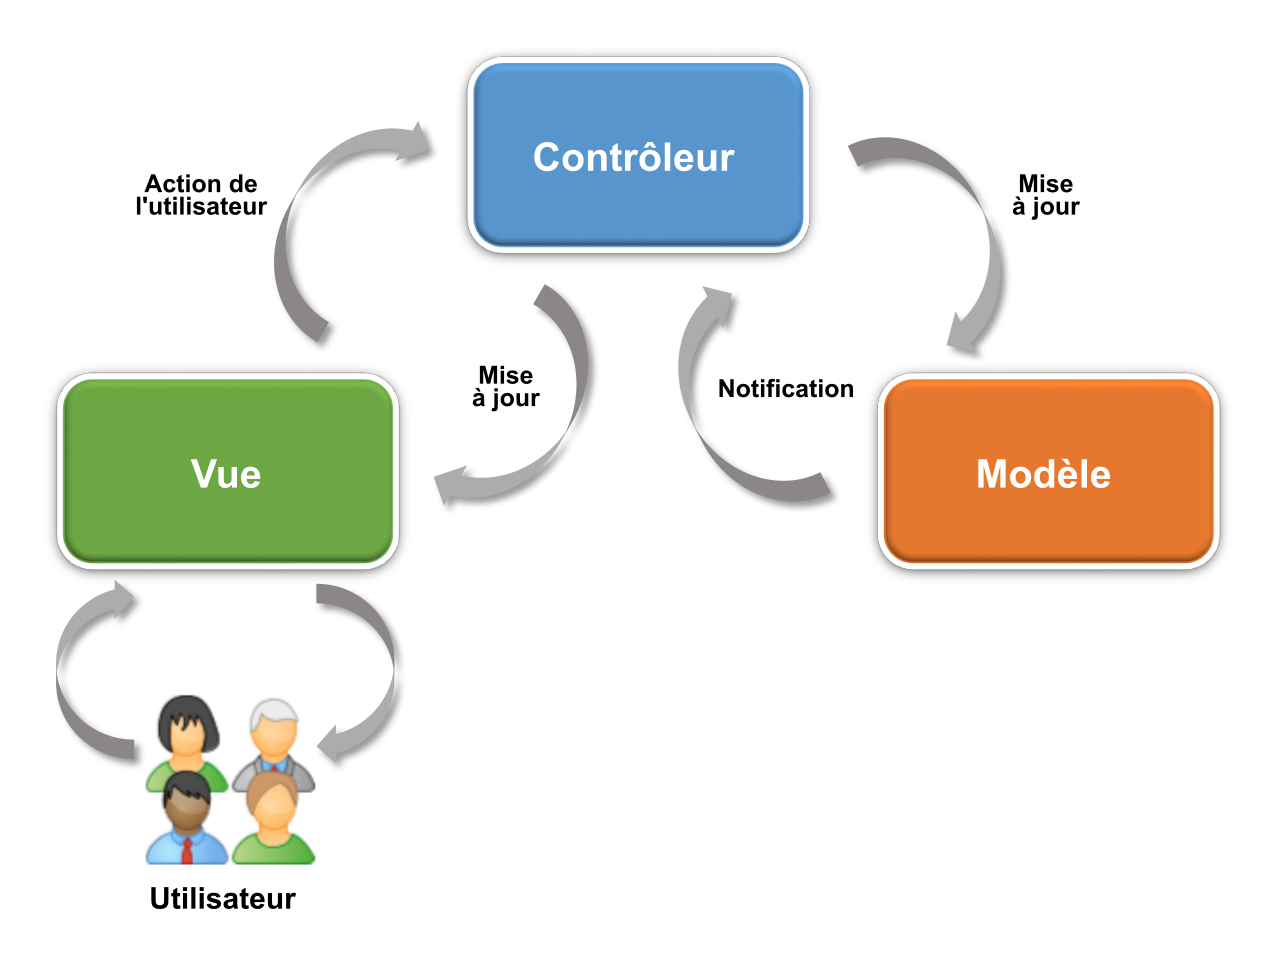
\includegraphics[width=\textwidth, height=0.3\textheight, keepaspectratio]{logos/mvc.png}
    \caption{Architecture de l'application JourneyBuddy (MVC)}
\end{figure}

\section{Conclusion}

L'analyse détaillée du projet JourneyBuddy a permis de définir les besoins fondamentaux, l’architecture technique, les outils à employer et les méthodes agiles à mettre en place. La combinaison de la stack MERN, de l’approche MVC, et de la gestion Scrum garantit une base solide pour assurer la réussite de l’application mobile.


% CHAPTER 3: Réalisation
\chapter{Réalisation}
\section{Introduction}

Ce chapitre présente les différentes itérations de développement du projet sous forme de \textbf{quatre sprints essentiels}, chacun correspondant à un ou plusieurs cas d'utilisation majeurs. Chaque sprint comprend les étapes de planification, conception, modélisation UML, et développement avec les interfaces graphiques correspondantes.

\section{Sprint 1 : Inscription, Authentification et Gestion de profil}

Ce premier sprint a pour objectif la mise en place des fonctionnalités fondamentales d'accès à l'application : inscription, authentification et gestion du profil utilisateur

\begin{table}[H]
\centering
\begin{tabularx}{\textwidth}{|c|l|l|X|c|}
\hline
\textbf{Sprint} & \textbf{User Story} & \textbf{En tant que} & \textbf{Je veux} & \textbf{Priorité} \\
\hline
Sprint 1 & Inscription & Voyageur & Créer un compte pour personnaliser mon expérience & Haute \\
\hline
Sprint 1 & Authentification & Voyageur & M’authentifier afin d’accéder à mon espace personnel. & Haute \\
\hline
Sprint 1 & Gestion de profil & Voyageur & Modifier mes informations de profil (photo, téléphone, ville/pays, bio, adresse, mot de passe) & Moyenne \\
\hline
\end{tabularx}
\caption{Sprint Backlog du Sprint 1}
\end{table}

% ================================
% 1) Use Case
% ================================
\subsection{Diagramme de cas d’utilisation du Sprint 1}

Ce diagramme illustre les interactions principales entre les acteurs et les fonctionnalités du sprint 1 (inscription, authentification et gestion du profil).

\begin{figure}[H]
    \centering
    \includegraphics[width=0.8\textwidth]{diagrams/usecases/profile.png}
    \caption{Diagramme de cas d'utilisation - Sprint 1}
\end{figure}

% ================================
% 2) Conception détaillée
% ================================
\subsection{Conception détaillée}

\subsubsection{Diagramme de classe}

Le diagramme de classe structure les entités principales impliquées dans les opérations d’identification et de gestion du profil utilisateur.

\begin{figure}[H]
    \centering
\includegraphics[width=0.95\textwidth]{diagrams/classes/profile.png}
    \caption{Diagramme de classe - Sprint 1}
\end{figure}


\subsubsection{Diagramme de séquence}

\subsubsubsection{Diagramme de séquence d'inscription}

Ce diagramme présente les échanges entre les objets du système lors du processus d’inscription d’un utilisateur.

\begin{figure}[H]
    \centering
    \includegraphics[width=0.85\textwidth]{diagrams/sequences/insc}
    \caption{Diagramme de séquence - Inscription}
\end{figure}

\subsubsection{Diagramme de séquence d'authentification}

Ce diagramme présente les échanges entre les objets du système lors du processus d’authentification d’un utilisateur.

\begin{figure}[H]
    \centering
    \includegraphics[width=\textwidth]{diagrams/sequences/auth.png}
    \caption{Diagramme de séquence - Authentification}

\end{figure}

\subsubsection{Diagramme de séquence de Gestion du Profile}

Ce diagramme présente les échanges entre les objets du système lors du processus de la gestion du profile.

\begin{figure}[H]
    \centering
    \includegraphics[width=0.85\textwidth]{diagrams/sequences/profile.png}
    \caption{Diagramme de séquence - Gestion du Profile}
\end{figure}

% ================================
% 3) Développement
% ================================
\subsection{Développement du Sprint 1}

Dans cette phase, les interfaces graphiques associées aux fonctionnalités du sprint sont développées. Elles permettent à l’utilisateur de s’inscrire, de s’authentifier et de gérer son profil de manière intuitive et sécurisée.

\begin{figure}[H]
    \centering
    \includegraphics[width=0.5\textwidth, keepaspectratio]{ui/begin/lancement.jpg}
    \caption{Interface graphique - Lancement de l'application}
\end{figure}

\begin{figure}[H]
    \centering
    \includegraphics[width=0.5\textwidth, keepaspectratio]{ui/begin/Explore.jpg}
    \caption{Interface graphique - Exploration de l'application}
\end{figure}

\begin{figure}[H]
    \centering
    \includegraphics[width=0.5\textwidth, keepaspectratio]{ui/begin/get_started.jpg}
    \caption{Interface graphique - Début de l'application}
\end{figure}

\begin{figure}[H]
    \centering
    \includegraphics[width=0.5\textwidth, keepaspectratio]{ui/begin/overboading1.jpg}
    \caption{Interface graphique - Le premier écran de démarrage de l'application}
\end{figure}


\begin{figure}[H]
    \centering
    \includegraphics[width=0.5\textwidth,keepaspectratio]{ui/begin/overboarding2.jpg}
    \caption{Interface graphique - Le deuxième écran de démarrage de l'application}
\end{figure}


\begin{figure}[H]
    \centering
    \includegraphics[width=0.5\textwidth, keepaspectratio]{ui/begin/overboarding3.jpg}
    \caption{Interface graphique - Le troisième écran de démarrage de l'application}
\end{figure}

\begin{figure}[H]
    \centering
    \includegraphics[width=0.5\textwidth, keepaspectratio]{ui/begin/overboarding4.jpg}
    \caption{Interface graphique - Le quatrième écran de démarrage de l'application}
\end{figure}

\begin{figure}[H]
    \centering
    \includegraphics[width=0.5\textwidth]{ui/begin/insc.jpg}
    \caption{Interface graphique - Formulaire d'inscription}
\end{figure}

\begin{figure}[H]
    \centering
     \includegraphics[width=0.5\textwidth]{ui/begin/fill_insc.jpg}
    \caption{Interface graphique - Remplissage du Formulaire d'inscription}
\end{figure}

\begin{figure}[H]
    \centering
    \includegraphics[width=0.5\textwidth]{ui/begin/login.jpg}
    \caption{Interface graphique - Formulaire d'authentification}
\end{figure}

\begin{figure}[H]
    \centering
     \includegraphics[width=0.5\textwidth]{ui/begin/fill_login.jpg}
    \caption{Interface graphique - Remplissage du Formulaire d'authentification}
\end{figure}
\newpage
\begin{figure}[H]
    \centering
    \includegraphics[width=0.5\textwidth]{ui/begin/login_home.jpg}
    \caption{Interface graphique - Interface Home}
\end{figure}

 
\begin{figure}[H]
    \centering
    \includegraphics[width=0.5\textwidth]{ui/settings/profile.jpg}
    \caption{Interface graphique -  profile}
\end{figure}

\begin{figure}[H]
    \centering
    \includegraphics[width=0.5\textwidth]{ui/settings/edit_profile.jpg}
    \caption{Interface graphique - Formulaire Modifier Profile}
\end{figure}

\begin{figure}[H]
    \centering
    \includegraphics[width=0.5\textwidth]{ui/settings/fill_profile.jpg}
    \caption{Interface graphique - Remplissage du Formulaire Profile }
\end{figure}

\begin{figure}[H]
    \centering
    \includegraphics[width=0.5\textwidth]{ui/settings/updated_profile.jpg}
    \caption{Interface graphique - Profile Modifié}
\end{figure}

% \begin{figure}[H]
%     \centering
%     \includegraphics[width=0.5\textwidth]{../ui/settings/password.jpg}
%     \caption{Interface graphique - Modifier Password}
% \end{figure}

% \begin{figure}[H]
%     \centering
%     \includegraphics[width=0.5\textwidth]{../ui/settings/update_password.jpg}
%     \caption{Interface graphique - Remplissage du Formulaire de Changer Password}
% \end{figure}

% \begin{figure}[H]
%     \centering
%     \includegraphics[width=0.5\textwidth]{../ui/settings/fill_password.jpg}
%     \caption{Interface graphique - Password Modifié}
% \end{figure}


% ================================
% Conclusion Sprint 1
% ================================
\subsection*{Conclusion du Sprint 1}

Le sprint 1 a permis de mettre en place les fonctionnalités essentielles d’accès à l’application, en intégrant à la fois la modélisation UML (cas d’utilisation, diagramme de classe et de séquence) et le développement des premières interfaces. Ces fondations assurent la continuité des prochains sprints.

% ================================
% Sprint 2
% ================================

\section{Sprint 2 : Création et Gestion de Voyage, Points d'intérêts et Alertes}

Ce deuxième sprint a pour objectif la mise en place des fonctionnalités principales liées à la gestion du voyage. 
Il permet aux utilisateurs de créer et gérer leurs voyages, de consulter des points d’intérêts, de gérer leurs favoris 
et de consulter les alertes disponibles dans l’application.

\usepackage{multirow} % add this in the preamble

\begin{table}[H]
\centering
\begin{tabular}{|c|l|l|l|c|}
\hline
\textbf{Sprint} & \textbf{User Story} & \textbf{En tant que} & \textbf{Je veux} & \textbf{Priorité} \\
\hline
\multirow{5}{*}{Sprint 2} & Création du voyage & Voyageur & Créer un voyage & Haute \\
\cline{2-5}
 & Gestion du voyage & Voyageur & Gérer mon voyage & Haute \\
\cline{2-5}
 & Consultation des points d'intérêts & Voyageur & Consulter des points d'intérêts & Moyenne \\
\cline{2-5}
 & Gestion des favoris & Voyageur & Gérer mes favoris & Moyenne \\
\cline{2-5}
 & Consultation des notifications internatiounaux culturels & Voyageur & Consulter des notifications internatiounaux culturels & Moyenne \\
\hline
\end{tabular}
\caption{Sprint Backlog du Sprint 2}
\end{table}


% ================================
% 1) Use Case
% ================================
\subsection{Diagramme de cas d’utilisation du Sprint 2}

Ce diagramme illustre les interactions principales entre les acteurs et les fonctionnalités du sprint 2 
(création et gestion de voyage, points d’intérêts, favoris et alertes).

\begin{figure}[H]
    \centering
    \includegraphics[width=0.85\textwidth]{diagrams/usecases/trip.png}
    \caption{Diagramme de cas d'utilisation - Sprint 2}
\end{figure}

% ================================
% 2) Conception détaillée
% ================================
\subsection{Conception détaillée}

\subsubsection{Diagramme de classe}

Le diagramme de classe structure les entités principales impliquées dans les opérations de gestion du voyage 
et des fonctionnalités associées (points d’intérêts, favoris, alertes).

\begin{figure}[H]
    \centering
    \includegraphics[width=0.95\textwidth]{diagrams/classes/trip.png}
    \caption{Diagramme de classe - Sprint 2}
\end{figure}

\subsubsection{Diagramme de séquence}

Ces diagrammes présentent les échanges entre les objets du système lors des processus de création et gestion d’un voyage, 
ainsi que la consultation des points d’intérêt et alertes.

\begin{figure}[H]
    \centering
    \includegraphics[width=0.85\textwidth]{trip}
    \caption{Diagramme de séquence - Création de voyage}
    
    \centering
    \includegraphics[width=0.85\textwidth]{recommandation .png}
    \caption{Diagramme de séquence - Recommandation des points d'intérêts }
    
    \centering
    \includegraphics[width=0.85\textwidth]{favoris.png}
    \caption{Diagramme de séquence - Gestion des favoris}
\end{figure}

% ================================
% 3) Développement
% ================================
\subsection{Développement du Sprint 2}

Dans cette phase, les interfaces graphiques associées aux fonctionnalités du sprint sont développées. 
Elles permettent à l’utilisateur de créer et gérer ses voyages, de consulter les points d’intérêts, de gérer ses favoris 
et de recevoir les alertes en toute simplicité.

\begin{figure}[H]
    \centering
    \includegraphics[width=0.6\textwidth]{ui_trip_creation}
    \caption{Interface graphique - Création d’un voyage}
    
    \centering  
    \includegraphics[width=0.6\textwidth]{ui_trip_management}
    \caption{Interface graphique - Gestion du voyage}
    
    \centering
    \includegraphics[width=0.6\textwidth]{ui_poi}
    \caption{Interface graphique - Consultation des points d’intérêts}
    
    \centering
    \includegraphics[width=0.6\textwidth]{ui_alerts}
    \caption{Interface graphique - Consultation les notifications internationaux culturels}
\end{figure}

% ================================
% Conclusion Sprint 2
% ================================
\subsection*{Conclusion du Sprint 2}

Le sprint 2 a permis de développer les fonctionnalités principales liées à la gestion de voyage, 
en intégrant la modélisation UML (cas d’utilisation, diagramme de classe et de séquence) et 
le développement des interfaces graphiques correspondantes. 
Il constitue une étape clé dans l’évolution de l’application en enrichissant considérablement l’expérience utilisateur.

% ================================
% Sprint 3
% ================================

\section{Sprint 3 : Recommandations AI et Chatbot}

Ce troisième sprint a pour objectif la mise en place des fonctionnalités intelligentes 
qui enrichissent l’expérience utilisateur. 
Il permet aux voyageurs de recevoir des recommandations personnalisées basées sur l’IA 
et d’interagir avec un chatbot pour obtenir de l’assistance ou des conseils de voyage en temps réel.

\begin{table}[H]
\centering
\begin{tabular}{|c|l|l|l|c|}
\hline
\textbf{Sprint} & \textbf{User Story} & \textbf{En tant que} & \textbf{Je veux} & \textbf{Priorité} \\
\hline
Sprint 3 & Consultation des recommandations AI & Voyageur & Consulter des recommandations personnalisées basées sur l’IA & Haute \\
\hline
Sprint 3 & Discussion avec un chatbot personnalisé & Voyageur & Discuter avec un chatbot intelligent pour obtenir de l’aide & Haute \\
\hline
\end{tabular}
\caption{Sprint Backlog du Sprint 3}
\end{table}

% ================================
% 1) Use Case
% ================================
\subsection{Diagramme de cas d’utilisation du Sprint 3}

Ce diagramme illustre les interactions principales entre les voyageurs et les fonctionnalités intelligentes du sprint 3 
(recommandations AI et chatbot).

\begin{figure}[H]
    \centering
    \includegraphics[width=0.85\textwidth]{chatbot}
    \caption{Diagramme de cas d'utilisation - Sprint 3}
\end{figure}

% ================================
% 2) Conception détaillée
% ================================
\subsection{Conception détaillée}

\subsubsection{Diagramme de classe}

Le diagramme de classe structure les entités principales impliquées dans la génération des recommandations 
et l’interaction avec le chatbot.

\begin{figure}[H]
    \centering
    \includegraphics[width=0.95\textwidth]{chatbot}
    \caption{Diagramme de classe - Sprint 3}
\end{figure}

\subsubsection{Diagramme de séquence}

Ces diagrammes présentent les échanges entre les objets du système lors des processus de recommandation AI 
et de dialogue avec le chatbot.

\begin{figure}[H]
    \centering
    \includegraphics[width=0.85\textwidth]{recommandation}
    \caption{Diagramme de séquence - Recommandations AI}
    
    \centering
    \includegraphics[width=0.85\textwidth]{chatbot}
    \caption{Diagramme de séquence - Interaction avec le chatbot}
\end{figure}

% ================================
% 3) Développement
% ================================
\subsection{Développement du Sprint 3}

Dans cette phase, les interfaces graphiques associées aux fonctionnalités intelligentes sont développées. 
Elles permettent à l’utilisateur de consulter facilement des recommandations personnalisées 
et d’interagir de manière fluide avec le chatbot.

\begin{figure}[H]
    \centering
    \includegraphics[width=0.85\textwidth]{ui_ai_recommendations}
    \caption{Interface graphique - Recommandations AI}
    
    \centering
    \includegraphics[width=0.85\textwidth]{ui_chatbot}
    \caption{Interface graphique - Chatbot personnalisé}
\end{figure}

% ================================
% Conclusion Sprint 3
% ================================
\subsection*{Conclusion du Sprint 3}

Le sprint 3 a introduit l’intelligence artificielle dans l’application, 
en intégrant à la fois les recommandations personnalisées et un chatbot interactif. 
Cette étape marque un tournant majeur dans l’évolution du projet, 
apportant une véritable valeur ajoutée à l’expérience utilisateur 
en rendant l’application plus intelligente et interactive.

% ================================
% Sprint 4
% ================================

\section{Sprint 4 : Finalisation UI/UX et Intégration Docker}

Ce quatrième sprint a pour objectif de peaufiner l’expérience utilisateur à travers la finalisation UI/UX et de garantir la portabilité et la mise en production fluide 
grâce à l’intégration Docker.  
Ces deux étapes viennent consolider le projet et assurer sa pérennité technique et ergonomique.

\begin{table}[H]
\centering
\begin{tabular}{|c|l|l|l|c|}
\hline
\textbf{Sprint} & \textbf{User Story} & \textbf{En tant que} & \textbf{Je veux} & \textbf{Priorité} \\
\hline
Sprint 4 & Avoir une expérience utilisateur optimisée & Voyageur & Naviguer dans l’application avec fluidité et cohérence visuelle & Haute \\
\hline
Sprint 4 & Déployer l’application dans un environnement stable & Développeur & Lancer l’application dans un conteneur portable et reproductible & Haute \\
\hline
\end{tabular}
\caption{Sprint Backlog du Sprint 4}
\end{table}

% ================================
% 1) Finalisation UI/UX
% ================================
\subsection{Finalisation UI/UX}

\textbf{Bienfaits :}
\begin{itemize}
    \item Amélioration de l’ergonomie générale et de la fluidité de navigation.
    \item Uniformisation du design (couleurs, polices, icônes) pour renforcer la cohérence visuelle.
    \item Expérience utilisateur simplifiée et adaptée à différents types d’écrans.
\end{itemize}

\textbf{Démonstration :}  
Les interfaces finales ci-dessous illustrent la cohérence graphique et l’ergonomie renforcée :

\begin{figure}[H]
    \centering
    \includegraphics[width=0.55\textwidth]{ui_final_dashboard}
    \caption{Interface finale - Tableau de bord utilisateur}
    
    \centering
    \includegraphics[width=0.55\textwidth]{ui_final_navigation}
    \caption{Interface finale - Navigation optimisée}
\end{figure}

% ================================
% 2) Intégration Docker
% ================================
\subsection{Intégration Docker}

\textbf{Bienfaits :}
\begin{itemize}
    \item Portabilité : l’application peut s’exécuter sur n’importe quel environnement supportant Docker.
    \item Reproductibilité : garantie que tous les développeurs et serveurs disposent du même environnement.
    \item Déploiement simplifié : automatisation de l’installation et de la configuration.
\end{itemize}

\textbf{Démonstration :}  
Les captures ci-dessous illustrent la mise en conteneur et le déploiement de l’application :

\begin{figure}[H]
    \centering
    \includegraphics[width=0.7\textwidth]{dockerfile}
    \caption{Exemple de Dockerfile utilisé pour la conteneurisation}
    
    \centering
    \includegraphics[width=0.7\textwidth]{docker_running}
    \caption{Application en cours d’exécution dans un conteneur Docker}
\end{figure}

% ================================
% Conclusion Sprint 4
% ================================
\subsection*{Conclusion du Sprint 4}

Le sprint 4 a permis de livrer une application complète, 
à la fois **ergonomique pour les utilisateurs finaux** et **robuste pour le déploiement technique**.  
La finalisation UI/UX a apporté une meilleure fluidité et une cohérence visuelle, 
tandis que l’intégration Docker a garanti la portabilité et la stabilité du projet.  
Ce sprint clôture le cycle de développement en assurant la qualité globale de l’application, 
prête à être utilisée et déployée dans des environnements variés.


\clearpage

\chapter*{Conclusion Générale}
\addcontentsline{toc}{chapter}{Conclusion Générale}
Ce rapport a documenté le processus de développement de l’application mobile \textbf{Trip Assistant}, depuis sa conception initiale jusqu’à son implémentation. Ce projet démontre comment l’intelligence artificielle peut être utilisée efficacement pour améliorer l’expérience de planification de voyage en offrant une assistance intelligente et personnalisée.

Au cours de ce projet, j’ai acquis une expérience précieuse en développement mobile, en intégration de l’IA et en conception d’expérience utilisateur. Les défis rencontrés ont été des occasions d’améliorer mes compétences en résolution de problèmes et d’approfondir ma connaissance des pratiques modernes en ingénierie logicielle.

L’application Trip Assistant représente non seulement une réussite technique, mais aussi une solution concrète aux difficultés rencontrées par les voyageurs. Les retours positifs des utilisateurs test confirment le potentiel de l’application pour rendre la planification de voyage plus efficace et agréable.

Ce projet a joué un rôle clé dans mon évolution en tant qu’ingénieur, en me permettant de transformer des savoirs théoriques en une application réelle.

\end{document}
